\documentclass[UTF8,zihao=-4,fontset=fandol]{ctexart}

\usepackage[a4paper,top=2.4cm,bottom=2.4cm,left=2.5cm,right=2.5cm]{geometry}
\usepackage{amsmath,amssymb,bm}
\usepackage{booktabs}
\usepackage{tabularx}
\usepackage{graphicx}
\usepackage{subcaption}
\usepackage{float}
\usepackage{enumitem}
\usepackage{xcolor}
\usepackage{hyperref}
\usepackage{fancyhdr}
\usepackage{titlesec}
\usepackage{tcolorbox}
\usepackage{caption}

\graphicspath{{paper/figures/}{figures/}}

\definecolor{OilBlue}{HTML}{1D4ED8}
\definecolor{OilRed}{HTML}{DC2626}
\definecolor{OilGreen}{HTML}{047857}
\definecolor{OilGray}{HTML}{374151}
\definecolor{OilLight}{HTML}{F8FAFC}

\hypersetup{
  colorlinks=true,
  linkcolor=OilBlue,
  urlcolor=OilBlue,
  citecolor=OilGreen,
  pdftitle={霍尔木兹海峡封锁对国际原油价格影响的短期动态模型研究},
  pdfauthor={数学建模 A 题项目组}
}

\pagestyle{fancy}
\fancyhf{}
\lhead{霍尔木兹海峡封锁与短期油价动态}
\rhead{\thepage}
\renewcommand{\headrulewidth}{0.4pt}
\setlength{\headheight}{15pt}

\titleformat{\section}{\Large\bfseries\color{OilBlue}}{\thesection}{0.6em}{}
\titleformat{\subsection}{\large\bfseries\color{OilGray}}{\thesubsection}{0.6em}{}
\captionsetup{font=small,labelfont=bf}
\setlist[itemize]{leftmargin=2em,itemsep=0.2em}
\setlist[enumerate]{leftmargin=2em,itemsep=0.2em}
\renewcommand{\arraystretch}{1.18}

\title{\bfseries 霍尔木兹海峡封锁对国际原油价格影响的短期动态模型研究}
\author{数学建模 A 题项目组}
\date{2026 年 5 月}

\begin{document}

\maketitle

\begin{abstract}
霍尔木兹海峡封锁会造成显著的原油运输中断。若直接采用静态供需弹性模型，油价上界容易被推高到远高于附件数据观测水平的区间。针对这一现象，本文以布伦特原油期货主力合约价格数据为基础，构建了一个用于解释冲突窗口短期油价演化的动态递推模型。模型将供应中断、战略石油储备释放、绕道运输恢复、商业库存缓冲、需求弹性调整、恐慌溢价、地缘风险溢价、缓冲确认折价和预期修复折价纳入统一框架，并通过固定种子多目标随机搜索与连续局部精修进行参数校准。结果表明，精修后的短期动态模型在冲突窗口内取得 RMSE 为 3.50 美元/桶、MAE 为 2.91 美元/桶的拟合效果；其中后期再定价 RMSE 为 2.99 美元/桶，低价回落区间 RMSE 为 3.51 美元/桶。模型不仅能解释价格冲击和高位平台，也能解释缓冲机制生效后的阶段性回落。该模型可作为后续 60--180 天情景预测与敏感性分析的中性基准。

\textbf{关键词：} 霍尔木兹海峡；原油价格；动态递推模型；战略石油储备；地缘风险；参数校准
\end{abstract}

\begin{tcolorbox}[colback=OilLight,colframe=OilBlue,title=核心结论]
传统静态供需模型给出的价格区间明显高估现实价格；加入库存、SPR、绕道、需求调整和预期修复后的短期动态模型，可以把冲突窗口油价解释到 110 美元/桶附近，并在后期回落段保持较低误差。
\end{tcolorbox}

\section{问题背景与建模思路}

霍尔木兹海峡是全球原油运输的关键咽喉。一旦发生封锁，直接影响不仅来自物理运输中断，也来自市场对未来供给安全的风险重估。若仅从短期供应减少出发，根据低弹性的需求曲线进行静态推算，模型会倾向于得到极高的油价上界。然而，附件数据中的冲突窗口价格主要处于 110--120 美元/桶附近，并未持续突破传统模型所推导出的高位区间。

这一差异说明，本题的关键不是简单回答“油价是否上涨”，而是解释：
\[
\text{巨大供应缺口} \quad \Longrightarrow \quad \text{为什么没有转化为同等幅度的持续价格暴涨？}
\]

已有油价冲击研究表明，原油价格变动通常包含供应冲击、需求冲击、库存调整、预防性需求和市场预期等多重因素。Kilian 的油价冲击分解研究强调，不同来源的油价冲击不能混为一谈；Kilian 与 Murphy 进一步指出，库存和投机性需求会影响现货油价。因此，本文将静态供需模型作为基准上界，再建立含多重缓冲机制的短期动态递推模型。

\section{数据说明与冲突窗口特征}

本文使用附件中的布伦特原油期货主力合约价格数据。阶段 1 对原始 CSV 进行了字段规范化、日期排序、收益率计算和冲突窗口截取。清洗后的全历史数据覆盖 2017 年 9 月 1 日至 2026 年 5 月 5 日；短期模型使用的冲突窗口为 2026 年 3 月 2 日至 2026 年 5 月 5 日，共 46 个实际交易日。

\begin{table}[H]
\centering
\caption{冲突窗口核心统计量}
\begin{tabular}{lr}
\toprule
指标 & 数值 \\
\midrule
交易日数 & 46 \\
窗口起始日 & 2026-03-02 \\
窗口终止日 & 2026-05-05 \\
最高收盘价 & 114.06 美元/桶 \\
最高盘中价 & 119.50 美元/桶 \\
模型校准目标 & 附件 CSV 的收盘价 \\
\bottomrule
\end{tabular}
\end{table}

\begin{figure}[H]
\centering

\includegraphics[width=0.95\linewidth]{price_trend.png}
\caption{布伦特原油期货主力合约长期价格走势。全历史图用于说明冲突窗口并非孤立数据，而是处于长期油价波动背景之中。}
\end{figure}

\begin{figure}[H]
\centering

\includegraphics[width=0.95\linewidth]{event_window_price.png}
\caption{2026 年冲突窗口内的实际油价走势。价格先快速上行，随后在高位震荡，并在中后期出现阶段性回落。}
\end{figure}

\section{传统供需基准模型}

首先建立传统静态供需模型作为上界对照。设战前日供给和需求均为 \(Q_0\)，封锁造成供应中断 \(\Delta Q\)，短期需求价格弹性为 \(\varepsilon_s < 0\)，基准价格为 \(P_0\)。在线性化近似下，价格相对变化可写为：
\begin{equation}
\frac{\Delta P}{P_0}
  \approx
  \frac{\Delta Q / Q_0}{|\varepsilon_s|}.
\end{equation}

由此得到的静态价格上界为：
\begin{equation}
P_{\mathrm{static}}
  =
  P_0
  \left(
  1 +
  \frac{\Delta Q / Q_0}{|\varepsilon_s|}
  \right).
\end{equation}

阶段 2 的基准模型结果表明，在题面供应中断量和短期低弹性假设下，传统供需模型会给出约 278--337 美元/桶的价格区间，明显高于附件数据中的最高收盘价 114.06 美元/桶。这说明静态供需模型可以作为“无缓冲机制”的理论上界，但不足以解释现实价格路径。

\begin{figure}[H]
\centering

\includegraphics[width=0.92\linewidth]{baseline_vs_actual.png}
\caption{传统供需基准模型与实际油价对比。静态模型显著高估现实价格，说明必须引入动态缓冲机制。}
\end{figure}

\section{短期动态递推模型}

\subsection{模型结构}

短期动态模型以日度为时间步长。设第 \(t\) 日模拟价格为 \(P_t\)，实际可用供给为 \(S_t\)，有效需求为 \(D_t\)，剩余供需缺口为 \(G_t\)。模型先计算供需侧变量，再将价格分解为基准价格、供需缺口压力、风险溢价、恐慌溢价和折价修复项。

有效供给由战前供给、供应中断、SPR 释放、绕道运输和库存缓冲共同决定：
\begin{equation}
S_t
  =
  Q_0
  -
  I
  +
  R_t^{\mathrm{SPR}}
  +
  R_t^{\mathrm{route}}
  +
  B_t^{\mathrm{inv}},
\end{equation}
其中 \(I\) 为供应中断量，\(R_t^{\mathrm{SPR}}\) 为战略石油储备释放量，\(R_t^{\mathrm{route}}\) 为绕道运输恢复量，\(B_t^{\mathrm{inv}}\) 为商业库存缓冲量。

有效需求考虑价格弹性和观察到的需求收缩：
\begin{equation}
D_t
  =
  Q_0
  \left(
  \frac{P_{t-1}}{P_0}
  \right)^{\varepsilon_t}
  -
  C_t,
\end{equation}
其中 \(\varepsilon_t\) 从短期低弹性逐步过渡到中长期弹性，\(C_t\) 表示高油价和冲击持续下的需求收缩。

剩余缺口为：
\begin{equation}
G_t = \max(D_t - S_t, 0).
\end{equation}

\subsection{价格递推方程}

模型将第 \(t\) 日目标价格写为：
\begin{equation}
P_t^{*}
=
P_0
+ \Phi_t^{\mathrm{gap}}
+ \Phi_t^{\mathrm{risk}}
+ \Phi_t^{\mathrm{uncertainty}}
+ \Phi_t^{\mathrm{panic}}
- \Psi_t^{\mathrm{buffer}}
- \Psi_t^{\mathrm{relief}}.
\end{equation}

其中，供需缺口压力项为：
\begin{equation}
\Phi_t^{\mathrm{gap}}
  =
  P_0
  \alpha
  \frac{G_t / Q_0}{|\varepsilon_t|},
\end{equation}
\(\alpha\) 为供需缺口压力系数。地缘风险溢价采用先上升后缓慢衰减的形式：
\begin{equation}
\Phi_t^{\mathrm{risk}}
  =
  P_0
  \beta
  \frac{I}{Q_0}
  \left(1-e^{-t/7}\right)e^{-\lambda t}.
\end{equation}

恐慌溢价由指数衰减的情绪因子表示：
\begin{equation}
\Phi_t^{\mathrm{panic}}
  =
  0.45P_0 f_0 e^{-\rho t}.
\end{equation}

为了刻画市场看到缓冲机制生效后的再定价过程，本文加入两类折价项。第一类为缓冲确认折价：
\begin{equation}
\Psi_t^{\mathrm{buffer}}
  =
  P_0 \eta
  \left(1-e^{-(t-\tau_b)/3}\right)
  e^{-(t-\tau_b)/d_b},
  \quad t \ge \tau_b.
\end{equation}
第二类为预期修复折价：
\begin{equation}
\Psi_t^{\mathrm{relief}}
  =
  P_0 \theta
  \min\left(
  \frac{t-\tau_s}{\tau_p-\tau_s}, 1
  \right)
  e^{-\max(t-\tau_p,0)/d_r},
  \quad t \ge \tau_s.
\end{equation}

最终模拟价格按照部分调整机制递推：
\begin{equation}
P_t
  =
  P_{t-1}
  +
  v(P_t^{*}-P_{t-1}),
\end{equation}
其中 \(v\) 为价格向目标价格调整的速度。

\section{参数校准与评价指标}

\subsection{多目标校准}

为避免模型只追求整体 RMSE 而牺牲峰值、末日价格或分段解释能力，本文采用多目标校准函数：
\begin{align}
\mathcal{L}
=&
\mathrm{RMSE}
+0.20|\Delta P_{\mathrm{peak}}|
+0.25|\Delta P_{\mathrm{final}}| \notag\\
&+0.15\mathrm{RMSE}_{\mathrm{high}}
+0.12\mathrm{RMSE}_{\mathrm{early}}
+0.12\mathrm{RMSE}_{\mathrm{mid}} \notag\\
&+0.18\mathrm{RMSE}_{\mathrm{late}}
+0.18\mathrm{RMSE}_{\mathrm{low}} .
\end{align}

其中 RMSE 和 MAE 定义为：
\begin{equation}
\mathrm{RMSE}
  =
  \sqrt{
  \frac{1}{n}
  \sum_{t=1}^{n}
  (P_t-\hat{P}_t)^2
  },
\qquad
\mathrm{MAE}
  =
  \frac{1}{n}
  \sum_{t=1}^{n}
  |P_t-\hat{P}_t|.
\end{equation}

参数校准分两步进行：第一步使用固定随机种子进行 36000 组多目标参数搜索，覆盖物理参数和行为参数的合理范围；第二步使用 SciPy 差分进化算法进行连续局部精修，使模型同时满足整体误差和分段误差要求。

\subsection{校准参数}

\begin{table}[H]
\centering
\caption{综合最优短期模型参数}
\begin{tabular}{lr@{\quad}lr}
\toprule
参数 & 数值 & 参数 & 数值 \\
\midrule
供应中断量 & 1482 & SPR 释放上限 & 674 \\
SPR 启动延迟 & 4 & 绕道启动日 & 10 \\
绕道能力上限 & 256 & 长期需求弹性 & -0.24 \\
恐慌初始强度 & 0.13 & 恐慌衰减速度 & 0.11 \\
库存日缓冲上限 & 282 & 调整速度 \(v\) & 0.342 \\
风险权重 \(\beta\) & 2.446 & 不确定性平台 & 0.244 \\
缓冲确认强度 \(\eta\) & 0.216 & 预期修复强度 \(\theta\) & 0.240 \\
\bottomrule
\end{tabular}
\end{table}

\section{结果分析}

\subsection{总体拟合效果}

综合最优模型在冲突窗口中取得 RMSE 为 3.50 美元/桶、MAE 为 2.91 美元/桶的拟合结果。模拟峰值为 110.31 美元/桶，实际最高收盘价为 114.06 美元/桶，峰值略低估 3.75 美元/桶；末日模拟价格与实际价格均为 110.31 美元/桶，说明模型在末端平台位置上具有较好稳定性。

\begin{figure}[H]
\centering

\includegraphics[width=0.95\linewidth]{短期模型拟合效果.png}
\caption{短期动态模型拟合效果。模型较好刻画了前期冲击、中期平台和后期再定价三个阶段。}
\end{figure}

\subsection{分段误差诊断}

\begin{table}[H]
\centering
\caption{短期动态模型分段误差}
\begin{tabular}{lrrrr}
\toprule
分段 & 样本数 & RMSE & MAE & 最大绝对误差 \\
\midrule
全窗口 & 46 & 3.50 & 2.91 & 7.21 \\
前期冲击 & 11 & 3.15 & 2.71 & 5.86 \\
中期平台 & 14 & 4.36 & 3.72 & 7.21 \\
后期再定价 & 21 & 2.99 & 2.47 & 5.35 \\
高价平台 & 4 & 2.74 & 2.22 & 3.95 \\
低价回落 & 21 & 3.51 & 3.08 & 5.86 \\
\bottomrule
\end{tabular}
\end{table}

分段误差表明，模型并非只在总体 RMSE 上表现较好。前期冲击、中期平台和后期再定价三个阶段的 RMSE 均保持在较低水平，尤其后期再定价 RMSE 仅为 2.99 美元/桶，说明缓冲确认折价和预期修复折价有效改善了原先后期回落解释不足的问题。

\begin{figure}[H]
\centering
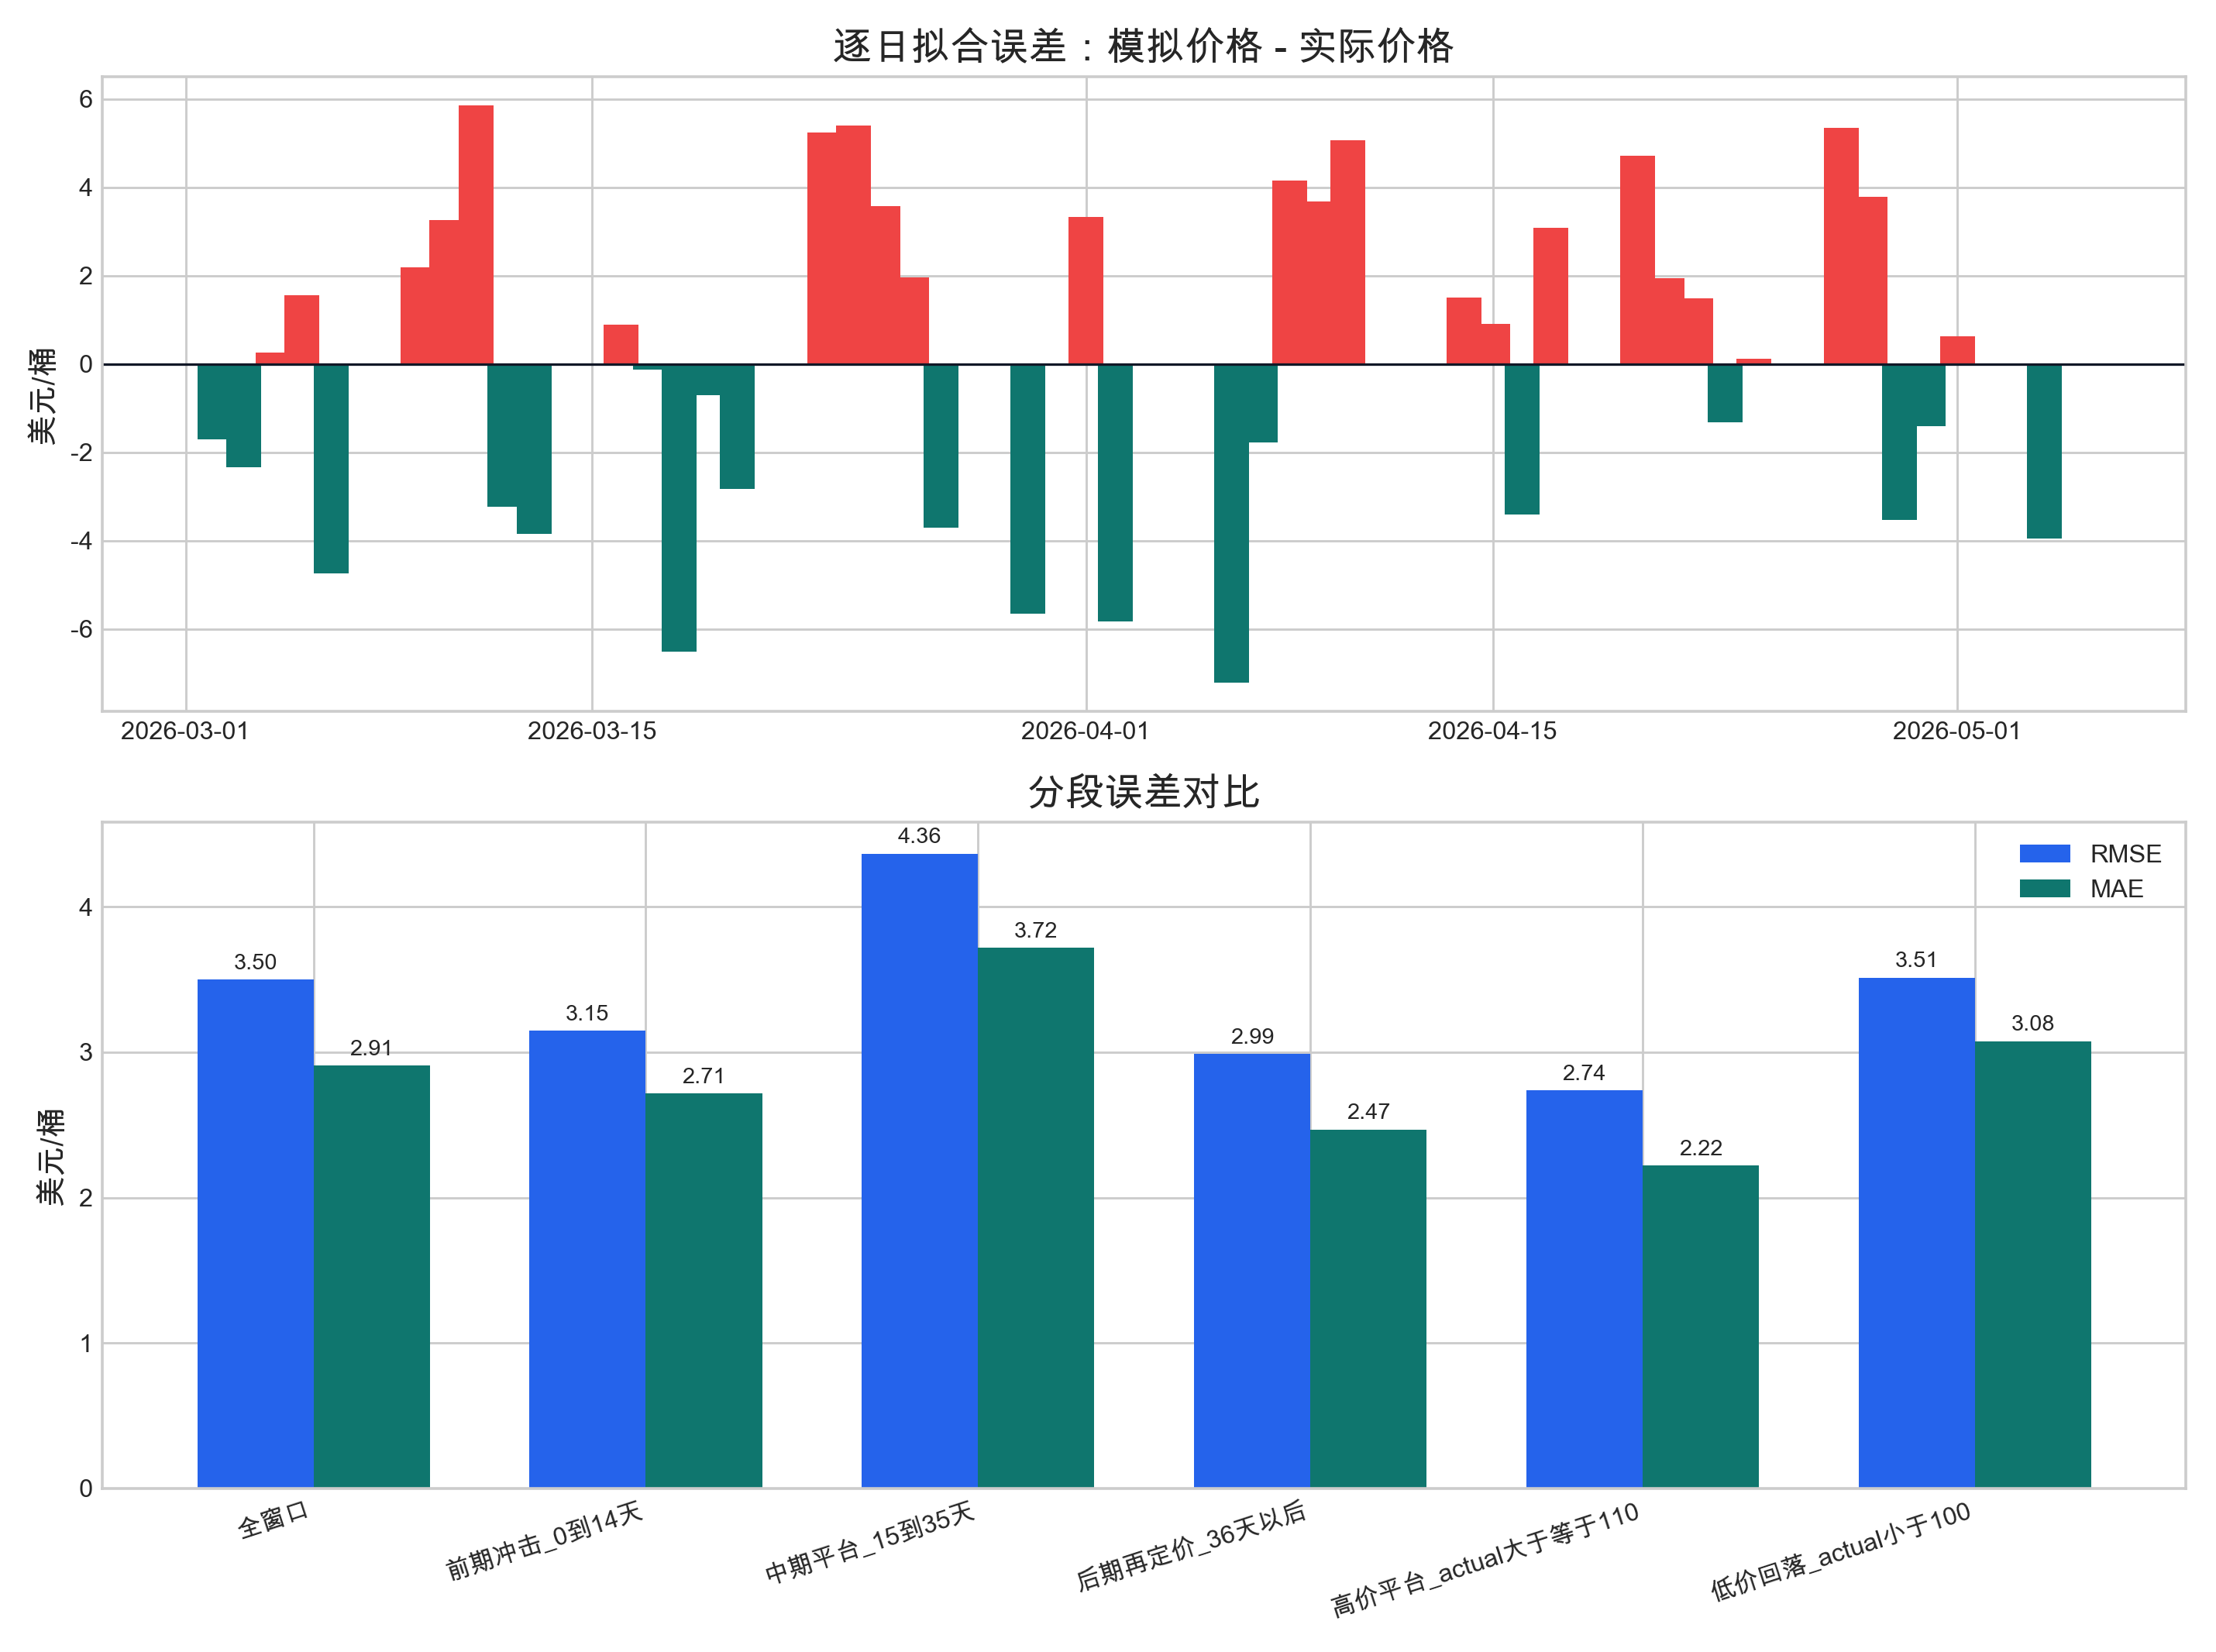
\includegraphics[width=0.95\linewidth]{短期模型误差诊断.png}
\caption{逐日误差与分段误差诊断。误差没有集中失控于某一阶段，说明模型具备较好的阶段稳健性。}
\end{figure}

\subsection{机制贡献解释}

机制贡献图显示，封锁风险溢价和不确定性溢价是价格维持高位的主要推升力量；恐慌溢价在前期较明显，但随时间快速衰减。中期以后，缓冲确认折价和预期修复折价逐步压低目标价格，解释了实际油价没有持续维持在极端高位的现象。

\begin{figure}[H]
\centering
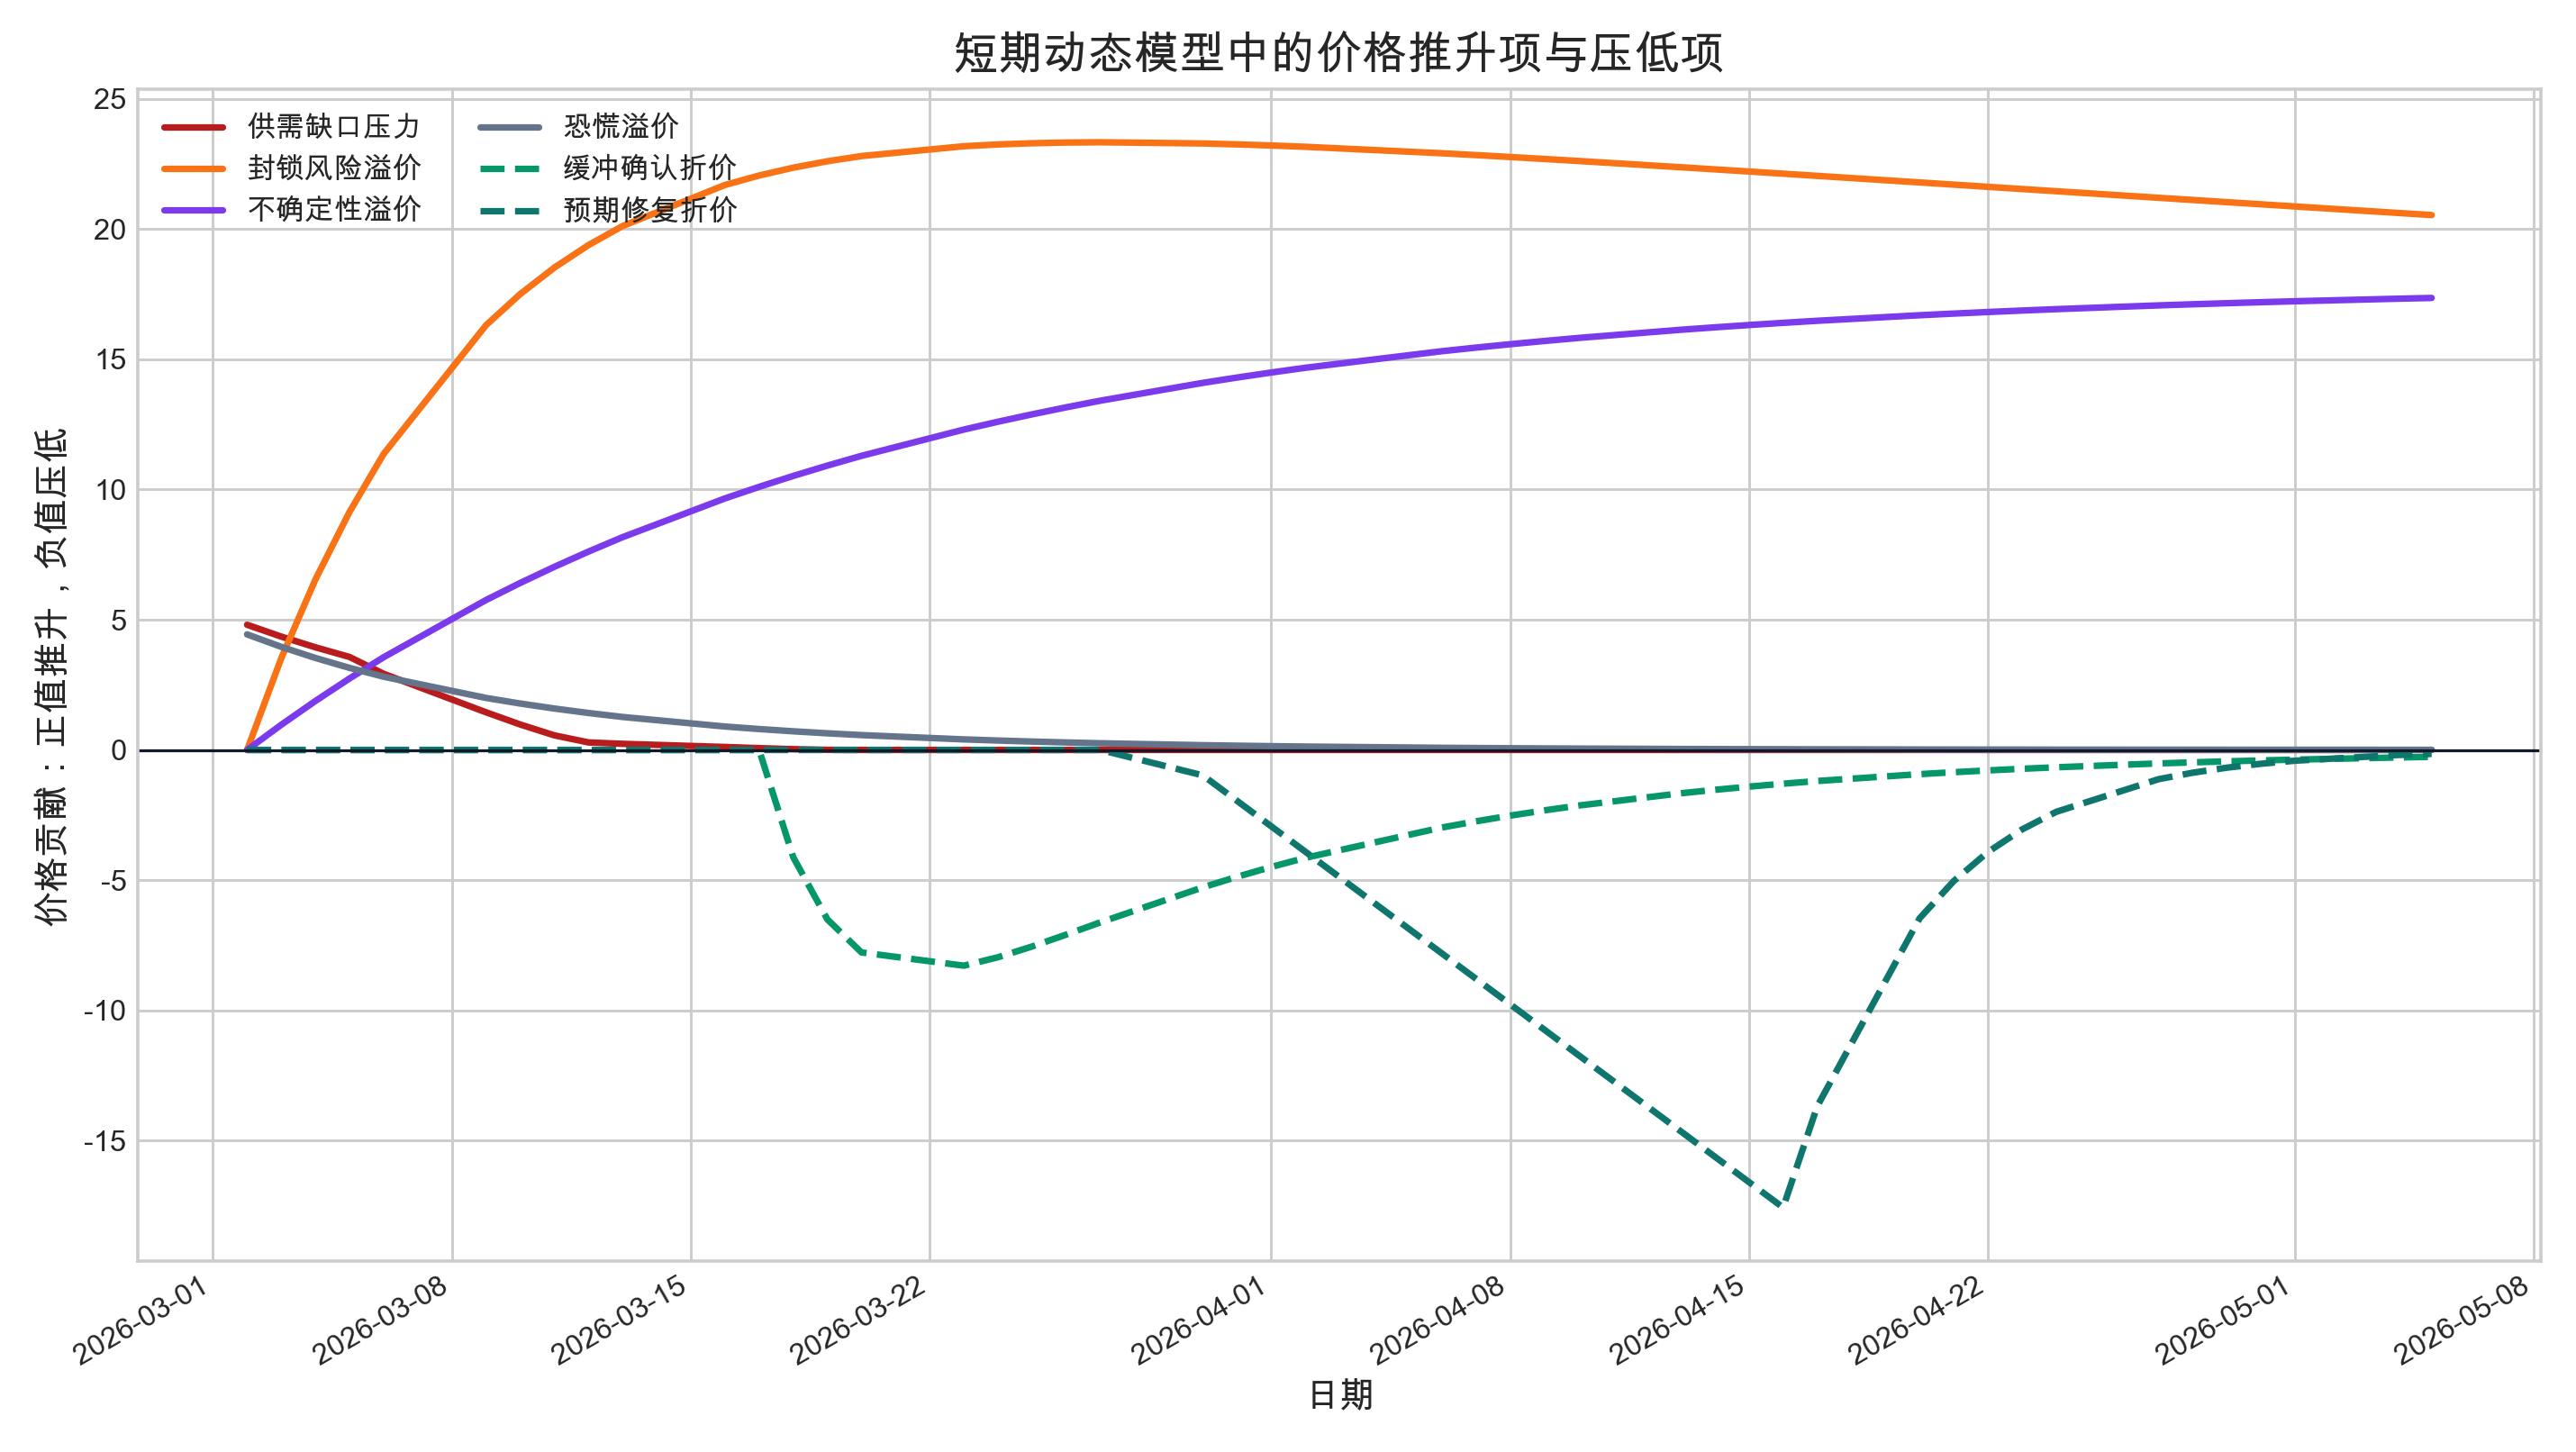
\includegraphics[width=0.95\linewidth]{短期模型机制贡献.png}
\caption{短期模型机制贡献分解。正值表示推升价格，负值表示压低价格。}
\end{figure}

\subsection{候选模型比较}

为了避免结论依赖单一参数组合，阶段 4 保留了综合最优、RMSE 最优、平台解释最优等候选模型。连续局部精修模型同时成为综合最优与 RMSE 最优；平台解释最优模型虽然对高价平台刻画更强，但整体误差和低价回落误差较高，因此不作为主模型。

\begin{figure}[H]
\centering
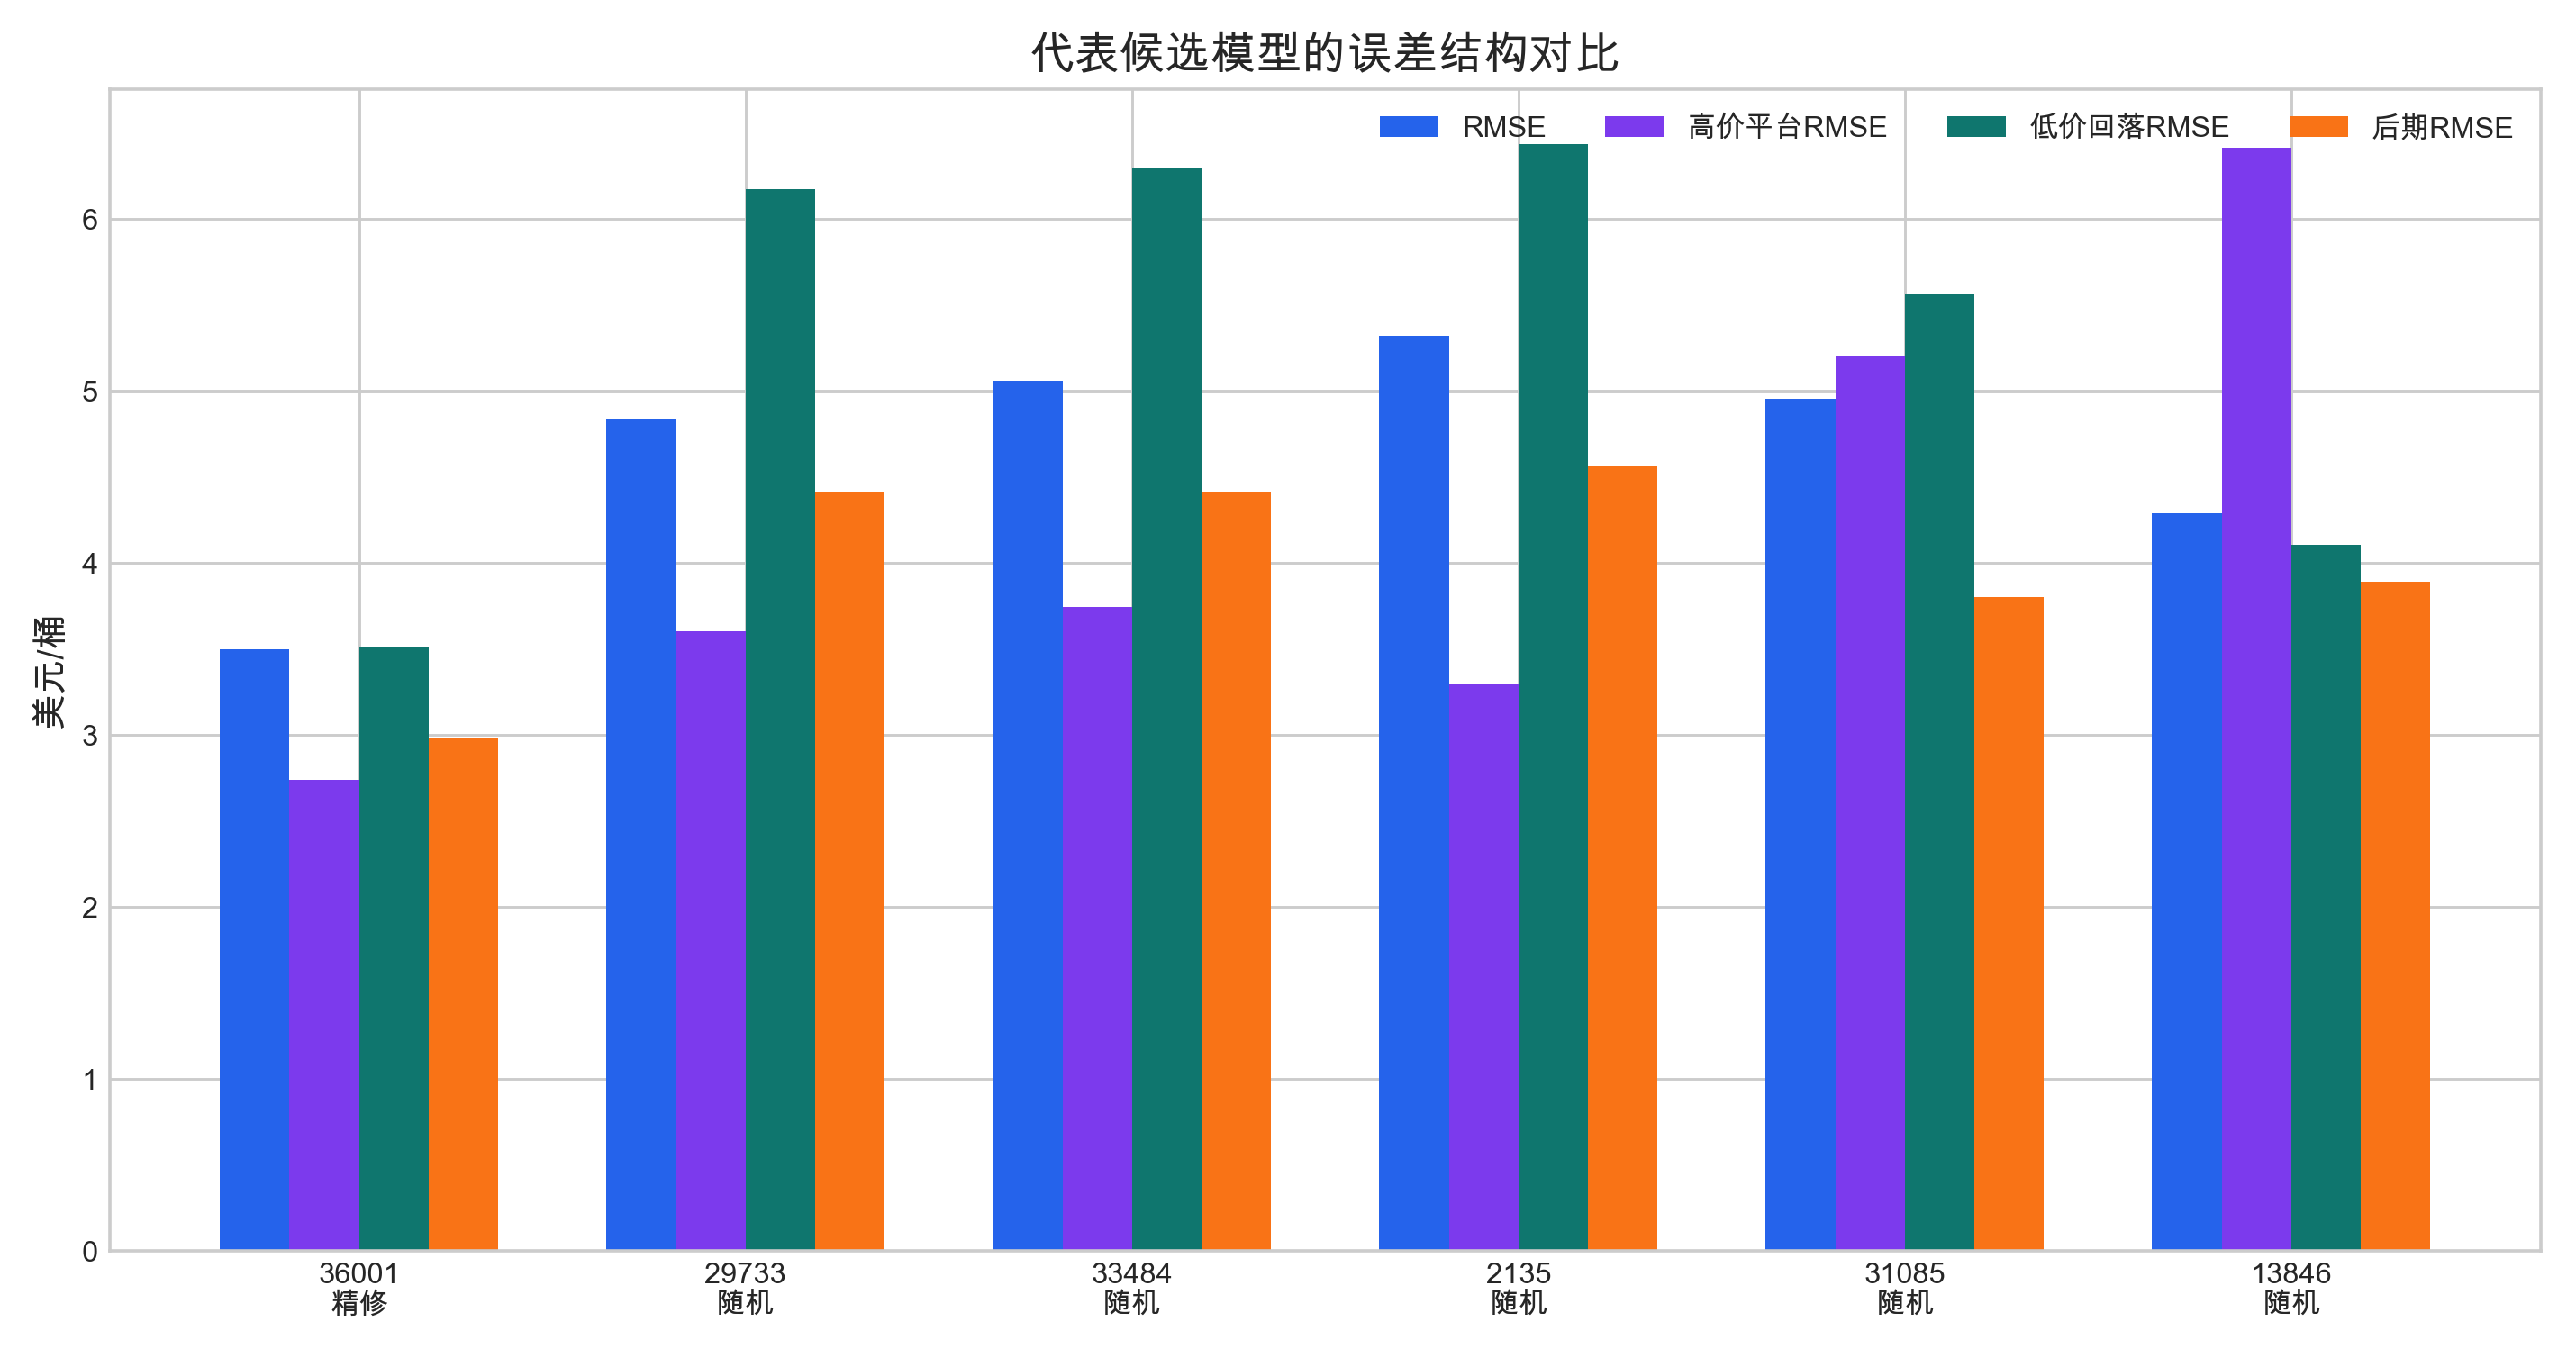
\includegraphics[width=0.92\linewidth]{候选模型误差对比.png}
\caption{代表候选模型误差结构对比。综合最优模型在整体误差、后期误差和低价回落误差之间取得更均衡的表现。}
\end{figure}

\section{模型评价与后续扩展}

本文短期动态模型具有三个优点。第一，模型结构与赛题机制对应明确，不是简单黑箱拟合；第二，模型通过多目标函数同时约束峰值、末日价格、平台误差和回落误差；第三，模型输出可以直接支撑后续三情景预测和敏感性分析。

模型也存在限制。首先，当前校准窗口只有 46 个交易日，样本规模较小；其次，地缘政治风险和市场预期以参数化方式进入模型，并未使用新闻文本或期权隐含波动率等外部变量；再次，本文聚焦短期窗口，尚未展开 60--180 天长期情景预测。

后续研究可在三个方向继续扩展：
\begin{enumerate}
  \item 基于当前综合最优参数，构建乐观、中性、悲观三类封锁持续情景；
  \item 对供应中断、SPR 释放、需求弹性和预期修复强度进行敏感性分析；
  \item 将阶段 4 的短期模型嵌入交互式展示系统，用于答辩演示和参数解释。
\end{enumerate}

\section{结论}

本文围绕霍尔木兹海峡封锁对国际原油价格的短期影响，建立了从静态供需上界到动态缓冲解释的模型链条。结果表明，传统供需模型能够说明供应缺口带来的理论价格压力，但会显著高估现实油价；加入战略储备、库存缓冲、绕道运输、需求弹性、地缘风险、恐慌衰减和预期修复后，短期动态模型能够较好解释冲突窗口内油价的上行、平台和回落。

校准结果显示，综合最优模型的全窗口 RMSE 为 3.50 美元/桶，MAE 为 2.91 美元/桶，后期再定价 RMSE 为 2.99 美元/桶，低价回落 RMSE 为 3.51 美元/桶。模型质量足以作为后续情景预测的中性基准，也可作为最终论文中短期机制解释部分的核心模型。

\begin{thebibliography}{99}
\bibitem{kilian2009}
Kilian, L. (2009). Not All Oil Price Shocks Are Alike: Disentangling Demand and Supply Shocks in the Crude Oil Market. \textit{American Economic Review}, 99(3), 1053--1069.

\bibitem{hamilton2009}
Hamilton, J. D. (2009). Causes and Consequences of the Oil Shock of 2007--08. \textit{Brookings Papers on Economic Activity}, Spring 2009, 215--261.

\bibitem{kilianmurphy2014}
Kilian, L., \& Murphy, D. P. (2014). The Role of Inventories and Speculative Trading in the Global Market for Crude Oil. \textit{Journal of Applied Econometrics}, 29(3), 454--478.

\bibitem{baumeisterkilian2016}
Baumeister, C., \& Kilian, L. (2016). Understanding the Decline in the Price of Oil since June 2014. \textit{Journal of the Association of Environmental and Resource Economists}, 3(1), 131--158.

\bibitem{caldara2022}
Caldara, D., \& Iacoviello, M. (2022). Measuring Geopolitical Risk. \textit{American Economic Review}, 112(4), 1194--1225.

\bibitem{cooper2003}
Cooper, J. C. B. (2003). Price elasticity of demand for crude oil: estimates for 23 countries. \textit{OPEC Review}, 27(1), 1--8.

\bibitem{stevenszhang2021}
Stevens, P., \& Zhang, D. (2021). The asymmetric impact of strategic petroleum reserve releases on crude oil prices. \textit{Energy Economics}, 102, 105474.

\bibitem{eia2024}
U.S. Energy Information Administration. World Oil Transit Chokepoints.
\url{https://www.eia.gov/international/analysis/special-topics/World_Oil_Transit_Chokepoints}
\end{thebibliography}

\end{document}
